\documentclass[letterpaper,10pt]{article}

\usepackage{geometry}
\usepackage{hyperref}
\usepackage{glossaries}
\usepackage[pdftex]{graphicx}
\usepackage{tikz}
\usepackage{wrapfig}
\geometry{textheight=8.5in, textwidth=6in}
\newenvironment{bottompar}{\par\vspace*{\fill}}{\clearpage}

\makeglossaries
\loadglsentries[main]{Glossary}

\title{Technical Review And Implementation Plan For RockSat-X Payload - Hephaestus}
\author{Helena~Bales, Amber~Horvath, and Michael~Humphrey\\ \\ CS461 - Fall 2016}

\parindent = 0.0 in
\parskip = 0.1 in

\begin{document}
\maketitle

\begin{abstract}
The \gls{osu} RockSat-X team shall be named Hephaestus.
The possible methods for implementing our project requirements shall be outlined in this document.
The mission requires that the \gls{payload}, an autonomous robotic arm, perform a series of motions to locate predetermined targets.
The hardware shall be capable of performing the motions to reach the targets.
The software shall determine the targets and send the commands to the hardware to execute the motion.
The combination of the hardware controlled by the software shall demonstrate Hephaestus's ability to construct small parts on orbit.
This document will focus on the implementation of the software, but shall include necessary project context including hardware.
\end{abstract}

\begin{bottompar}
Approved By
\_\_\_\_\_\_\_\_\_\_\_\_\_\_\_\_\_\_\_\_\_\_\_\_\_\_\_\_\_\_\_\_\_\_\_\_\_\_\_\_\_\_\_\_\_\_\_\_\_\_\_\_\_\_\_\_\_\_\_\_\_\_\_
Date \_\_\_\_\_\_\_\_\_\_\_\_\_\_\_\_\_\_\_\_\_\_\_\_\_\_\_\_ \\


Approved By
\_\_\_\_\_\_\_\_\_\_\_\_\_\_\_\_\_\_\_\_\_\_\_\_\_\_\_\_\_\_\_\_\_\_\_\_\_\_\_\_\_\_\_\_\_\_\_\_\_\_\_\_\_\_\_\_\_\_\_\_\_\_\_
Date \_\_\_\_\_\_\_\_\_\_\_\_\_\_\_\_\_\_\_\_\_\_\_\_\_\_\_\_ \\


Approved By
\_\_\_\_\_\_\_\_\_\_\_\_\_\_\_\_\_\_\_\_\_\_\_\_\_\_\_\_\_\_\_\_\_\_\_\_\_\_\_\_\_\_\_\_\_\_\_\_\_\_\_\_\_\_\_\_\_\_\_\_\_\_\_
Date \_\_\_\_\_\_\_\_\_\_\_\_\_\_\_\_\_\_\_\_\_\_\_\_\_\_\_\_ \\


Approved By
\_\_\_\_\_\_\_\_\_\_\_\_\_\_\_\_\_\_\_\_\_\_\_\_\_\_\_\_\_\_\_\_\_\_\_\_\_\_\_\_\_\_\_\_\_\_\_\_\_\_\_\_\_\_\_\_\_\_\_\_\_\_\_
Date \_\_\_\_\_\_\_\_\_\_\_\_\_\_\_\_\_\_\_\_\_\_\_\_\_\_\_\_ \\
\end{bottompar}

\clearpage
\tableofcontents
\clearpage

\section{Introduction}
\subsection{Document Overview}
This is the Technical Review And Implementation Plan for the Hephaestus project.
This document shall investigate possible methods of implementing our project software requirements.
The nine general requirements investigated below were identified as project requirements in our Requirements document.
This document will focus on the "how" of our requirements implementation.
\subsection{Role Breakdown}
Each CS Senior Design team member shall be responsible for ensuring the completion of the three items
from the requirements document that are assigned to them below.
\subsubsection{Helena Bales}
\begin{enumerate}
\item{Target Generation}
\item{Arm Movement}
\item{Arm Position Tracking}
\end{enumerate}
\subsubsection{Amber Horvath}
\begin{enumerate}
\item{Emergency Payload Expulsion}
\item{Program Modes of Operation}
\item{Target Success Sensors}
\end{enumerate}
\subsubsection{Michael Humphrey}
\begin{enumerate}
\item{Telemetry}
\item{Video Camera}
\item{Data Visualization and Processing}
\end{enumerate}

\section{Technologies}
\subsection{Target Generation}
\subsubsection{Requirement Overview}
The software shall generate points to be used in testing the Hephaestus arm.
The points will constitute the total test of the arm, and should therefore include points
representative of standard and edge cases.
These points shall be used as targets for the arm body.
\subsubsection{Proposed Solutions}
\begin{enumerate}
\item{
\textbf{The points shall be generated in 3-D polar form}, including an angle from normal, a radius, 
and a height. 
The angle shall be in the range of 0 and 359 degrees.
An angle of zero degrees shall be in the direction of payload deployment.
The radius shall be the distance from the arm's attachment to the base to the generated point.
The height of the point, for the purpose of target generation, shall be constant.
However the points will always be stored in a triple of angle from normal (\(\theta\)), radius (\(r\)), and height (\(h\)).
}
\item{
\textbf{The points shall be generated in 3-D Cartesian form}, including \(x\) position to the right 
or left of the \(y-axis\), the \(y\) position above or below the \(x-axis\), and the height, \(h\), 
above the \(xy-plane\).
Let the \(y-axis\) be the direction that the payload deploys from the can.
Let the \(x-axis\) be the perpendicular to the \(y-axis\) at the point where the arm is mounted 
to the rotating plate. 
Let \(h\) be the height above the \(xy-plane\), where the arm is attached to the rotating plate.
}
\item{
\textbf{The points shall be generated in 2-D Polar coordinates}, where the implementation is the 
same as described in the 3-D Polar coordinate section, with the exception of \(h\).
In this case, there shall be no \(h\).
The position can be represented in 2-D Polar coordinates on the plane of the base plate.
For the purpose of compatibility with the position of the arm, the height could be assumed to be 0.
}
\end{enumerate}

\subsection{Arm Movement}
\subsubsection{Requirement Overview}
The software shall control the movement of the arm body assembly. 
The position of the tip of the arm shall be tracked in the coordinate notation described in section 2.2 above.
The software shall rotate the arm body assembly in a full 360 degrees.
The software shall additionally control the movement the height of the arm body assembly.
The arm should descend and touch the baseplate of the payload at any rotation.
\subsubsection{Proposed Solutions}
\begin{enumerate}
\item{
\textbf{The movement of the arm shall be generated by a custom system where the movement of the arm is 
generated based on the current position and the starting position.} 
The position of the tip of the arm shall be stored as decided from the list of solutions above. 
In the case of the selection of solution 3, the position will have an added height. 
The position shall be denoted as point \(p\) and shall be the location of the tip of the arm.
The arm shall generate a series of commands for the motors to perform to go from \(p\) to the target, 
\(t_{n}\) where \(t_{n}\) is the n-th target.
}

\item{
\textbf{The movement of the arm shall be generated by a custom system where the movement of the arm is 
generated based on the current position and the starting position.} 
The position of the tip of the arm shall be stored as decided from the list of solutions above. 
In the case of the selection of solution 3, the position will have an added height. 
The position shall be denoted as point \(p\) and shall be the location of the tip of the arm.
The arm shall generate a series of commands for the motors to perform to go from \(p\) to the target, 
\(t_{n}\) where \(t_{n}\) is the n-th target.
The movement of the arm shall be constrained by the heights of the arm so that it will not collide with 
the top or base plates.
}

\item{
\textbf{The movement of the arm shall be accomplished by turning the arm to the correct \(\theta\), then correct radius, then correct height.}
The rotating base plate will be responsible for turning the arm to the correct \(\theta\) value.
The motors, labeled \(m1\), and \(m2\), shall be responsible for moving the arm to the correct radius and
 height. The position of the arm, \(p\), and the target position \(t_{n}\), shall be stored in the 
manner described in the section titled Arm Position Tracking.
}
\end{enumerate}

\begin{center}
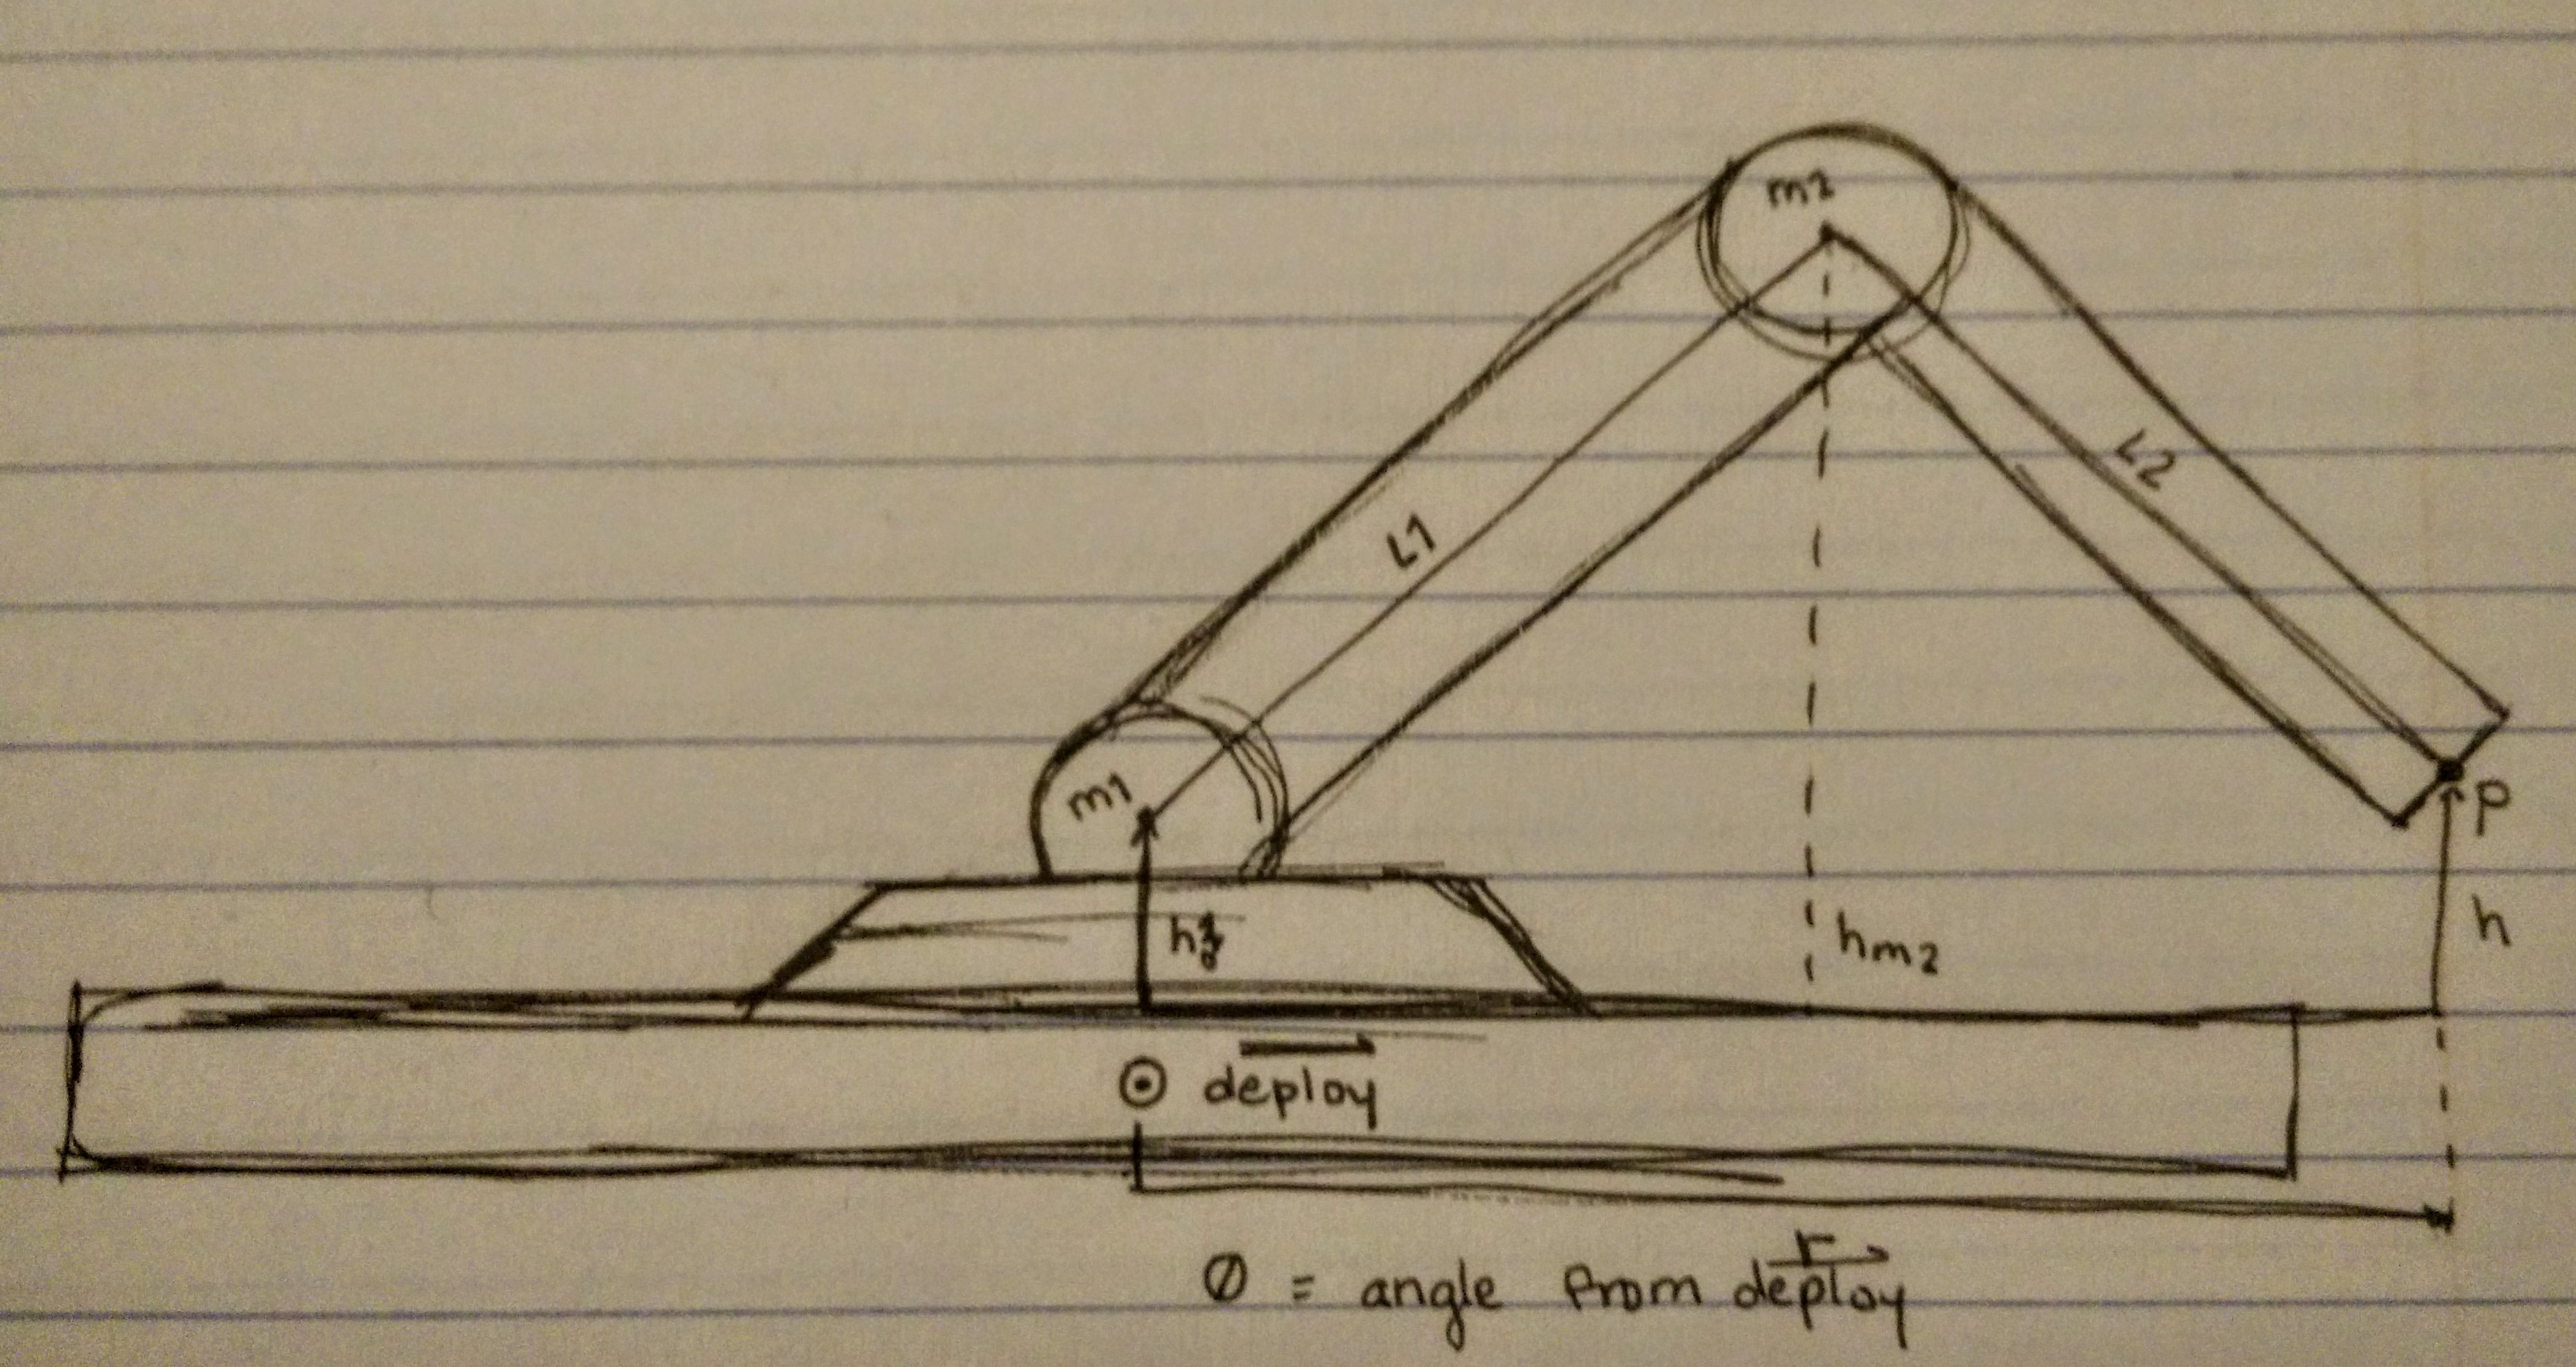
\includegraphics[width=\textwidth]{armDiagram}
\textbf{Figure 1} -- Arm Movement Design
\end{center}

\subsection{Arm Position Tracking}
\subsubsection{Requirement Overview}
The position of the arm shall be tracked using the same coordinate system described in the Target Generation requirement.
The position of the arm shall be calculated using the known start position and the rotation of the motors.
The starting position shall be known due to a calibration point that will allow for a reset at any time.
Resetting in this way will allow for flexibility between resetting for maximum operation time with only tolerably small error defined by the Non Functional Requirements.
\subsubsection{Proposed Solutions}
\begin{enumerate}
\item{
\textbf{The position of the arm shall be tracked using the motor movement.}
The initial position of the arm shall be defined in advance, and a sensor will be placed at that location. 
From there, the position will be tracked from the movement of the motors.
The arm will recalibrate by returning to the initial position in order for the error to not increase over
 time.
The position of the arm shall be denoted \(p\), the location of the tip of the arm.
This shall be the only position tracked.
}
\item{
\textbf{The position of the arm shall be tracked using the motor movement to calculate \(p\) and 
\(p_{m2}\).}
The initial position of the arm shall be defined in advance, and a sensor will be placed at that location. 
From there, the position will be tracked from the movement of the motors.
The arm will recalibrate by returning to the initial position in order for the error to not increase over
 time.
The position of the arm shall be denoted \(p\), the location of the tip of the arm.
From the coordinate \(p\), the location of \(p_{m2}\), the center of the middle joint of the arm, will be
 calculated. The height of \(p_{m2}\) will be calculated from the triangle made of the two arm sections, 
L1 and L2, and the radius of point \(p\). From there the radius of the point \(p_{m2}\) can be calculated
 using the triangle of L1, \(h_{m2}\) and the radius of m2. Finally, the \(\sigma\) of \(p_{m2}\) shall 
be the same as that of \(p\).
Using this method will allow for the extra condition that point \(p_{m2}\) should never exceed the height
 of the can.
}
\item{
\textbf{The position of the arm shall be tracked using the motor movement to calculate \(p\), with a
 limit on the height of the arm.}
The initial position of the arm shall be defined in advance, and a sensor will be placed at that location. 
From there, the position will be tracked from the movement of the motors.
The arm will recalibrate by returning to the initial position in order for the error to not increase over
 time.
The position of the arm shall be denoted \(p\), the location of the tip of the arm.
This will be the only point tracked, however the values of \(p\) shall be restricted such that the 
height of the arm never exceeds the height of our half can.
}


\end{enumerate}

\subsection{Emergency Payload Expulsion}
\subsubsection{Requirement Overview}
\subsubsection{Proposed Solutions}
\subsection{Program Modes of Operation}
\subsubsection{Requirement Overview}
The Software shall have the Modes of Operation necessary to insure the mission success.
The software shall first deploy the payload, then the arm. Next the software shall activate the 
camera and perform a video sweep. The software shall then perform the science experiment.
If the experiment fails, it shall return to observation mode.
If observation mode fails, it shall return to idle.
Once the experiment time has been exhausted, the payload shall shut down.
If it shuts down correctly, everything will poweroff. If not, the payload shall attempt to retract 
again, or expel the payload from the rocket.
\subsubsection{Proposed Solutions}
\begin{center}
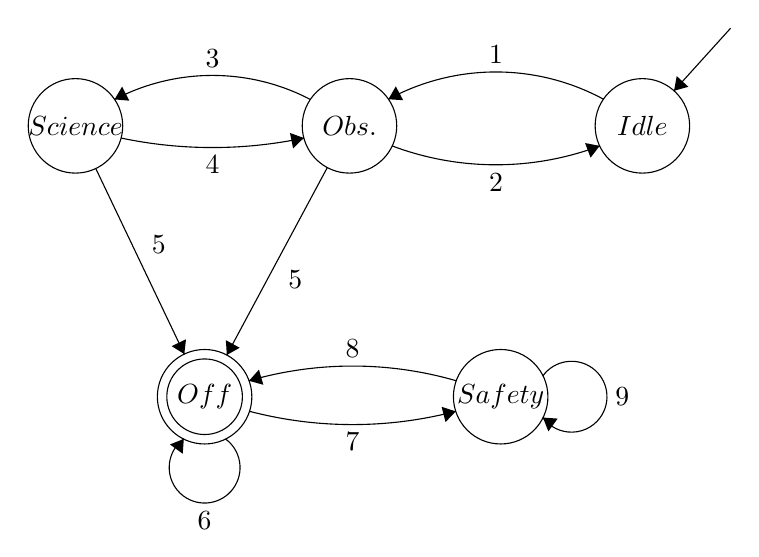
\begin{tikzpicture}[scale=0.2]
\tikzstyle{every node}+=[inner sep=0pt]
\draw [black] (24.2,-19.2) circle (3);
\draw (24.2,-19.2) node {$Obs.$};
\draw [black] (42.8,-19.2) circle (3);
\draw (42.8,-19.2) node {$Idle$};
\draw [black] (6.8,-19.2) circle (3);
\draw (6.8,-19.2) node {$Science$};
\draw [black] (15,-36.4) circle (3);
\draw (15,-36.4) node {$Off$};
\draw [black] (15,-36.4) circle (2.4);
\draw [black] (33.8,-36.4) circle (3);
\draw (33.8,-36.4) node {$Safety$};
\draw [black] (48.4,-13) -- (44.81,-16.97);
\fill [black] (44.81,-16.97) -- (45.72,-16.72) -- (44.98,-16.04);
\draw [black] (26.67,-17.507) arc (118.43354:61.56646:14.344);
\fill [black] (26.67,-17.51) -- (27.61,-17.57) -- (27.14,-16.69);
\draw (33.5,-15.28) node [above] {$1$};
\draw [black] (40.088,-20.475) arc (-69.41442:-110.58558:18.736);
\fill [black] (40.09,-20.47) -- (39.16,-20.29) -- (39.51,-21.22);
\draw (33.5,-22.17) node [below] {$2$};
\draw [black] (9.281,-17.525) arc (117.61533:62.38467:13.416);
\fill [black] (9.28,-17.52) -- (10.22,-17.6) -- (9.76,-16.71);
\draw (15.5,-15.5) node [above] {$3$};
\draw [black] (21.303,-19.973) arc (-78.10445:-101.89555:28.152);
\fill [black] (21.3,-19.97) -- (20.42,-19.65) -- (20.62,-20.63);
\draw (15.5,-21.08) node [below] {$4$};
\draw [black] (8.09,-21.91) -- (13.71,-33.69);
\fill [black] (13.71,-33.69) -- (13.82,-32.75) -- (12.91,-33.19);
\draw (11.61,-26.74) node [right] {$5$};
\draw [black] (16.323,-39.08) arc (54:-234:2.25);
\draw (15,-43.65) node [below] {$6$};
\fill [black] (13.68,-39.08) -- (12.8,-39.43) -- (13.61,-40.02);
\draw [black] (22.79,-21.85) -- (16.41,-33.75);
\fill [black] (16.41,-33.75) -- (17.23,-33.29) -- (16.35,-32.81);
\draw (20.28,-28.97) node [right] {$5$};
\draw [black] (30.948,-37.326) arc (-75.33467:-104.66533:25.865);
\fill [black] (30.95,-37.33) -- (30.05,-37.04) -- (30.3,-38.01);
\draw (24.4,-38.67) node [below] {$7$};
\draw [black] (17.821,-35.385) arc (106.14932:73.85068:23.653);
\fill [black] (17.82,-35.39) -- (18.73,-35.64) -- (18.45,-34.68);
\draw (24.4,-33.95) node [above] {$8$};
\draw [black] (36.48,-35.077) arc (144:-144:2.25);
\draw (41.05,-36.4) node [right] {$9$};
\fill [black] (36.48,-37.72) -- (36.83,-38.6) -- (37.42,-37.79);
\end{tikzpicture}
\end{center}
\begin{center}
Diagram of software states of operation and transition between states [2].

Transitions between states occur as numbered:

\begin{enumerate}
\item{\textbf{Appogee is reached.} The software shall activate when the power line goes to high at 28V. Observation mode shall be triggered when the OBC turns on.}
\item{\textbf{Error: Return to Idle.} If an error is encountered in entering Observation mode, the software shall fallback to Idle mode and retry. An error may occur if the payload fails to deploy correctly or if the camera fails to turn on.}
\item{\textbf{Payload Assembly and Camera have been deployed.} The software shall enter science mode once the payload assembly and arm have deployed and the camera has performed an observation sweep.}
\item{\textbf{Error: Return to Observation} The software shall return to observation mode if any error occurs in Science mode. An error may occur in Science mode if the arm fails to operate correctly and must return to default position. An error may also occur if the camera stops working.}
\item{\textbf{Timer switches to end appogee period.} Once the time period for observation has ended, the timer line will go to low and trigger to Shutdown state. This state can be reached from either Observation or Science mode.}
\item{\textbf{Accept: Shutdown correctly} If Shutdown occurs correctly, the arm should be closed, the Arm Assembly Body should be retracted, and the OBC should be powered off.}
\item{\textbf{Error: Shutdown not completed successfully.} If an error occurs in the shutdown sequence, the software shall enter Safety mode.}
\item{\textbf{Payload is Shutdown correctly.} If the payload is Shutdown through Safety mode, shutdown can be completed. In Safety mode the payload was either shut down correctly, retracted fully into the can with the arm open, or the arm was expelled safely from the rocket.}
\item{\textbf{Error: Shutdown not completed successfully.} If an error occurs in the shutdown sequence, the software shall enter Safety mode.}
\item{\textbf{Payload is Shutdown correctly.} If the payload is Shutdown through Safety mode, shutdown can be completed. In Safety mode the payload was either shut down correctly, retracted fully into the can with the arm open, or the arm was expelled safely from the rocket.}
\item{\textbf{Error: Payload is still deployed.} The software shall remain in Safety mode until the payload is either retracted correctly, retracted fully with the arm in the open position, or ejected safely from the rocket. Safety mode shall first try to correctly retract the arm, then retract with the arm open, then repeat attempting ejection until the payload is ejected.}
\end{enumerate}
\end{center}

\subsection{Target Success Sensors}
\subsubsection{Requirement Overview}
\subsubsection{Proposed Solutions}

\subsection{Telemetry}
\subsubsection{Requirement Overview}
The software shall report via telemetry all sensor data.

The criteria that these technologies will be evaluated on is:
\begin{itemize}
\item \textbf{Ease of use.}
The chosen solution should let the developers focus on writing code and not encoding data for telemetry transmission.
Ideally, sending data through one of the telemetry ports should be no more than one line of code. 
\item \textbf{Reliability.}
The chosen solution should be able to relay 100\% of transmitted data to the ground station without corrupting or losing any of it.
\item \textbf{Documentation.}
The chosen solution should be well documented.
The developers should be able to quickly and easily locate supporting documentation for using the technology.
\item \textbf{Compatibility.}
The chosen solution should be compatible with the software and hardware of the \gls{payload}.
\end{itemize}

\subsubsection{Proposed Solutions}
The three options being considered for transmitting telemetry are
\begin{enumerate}
\item{
\textbf{A custom-built solution for our own needs}.
The custom-built solution is the least appealing. It would require the most amount of work to develop and maintain by the developers.
The advantage of a custom-built solution is that it can be tailored to the requirements of our system, making it extremely to use.
However, the benefit is offset by the huge amount of work upfront it would require to develop and test the solution.
Since the developers would be coding up this solution themselves, it would require a lot of testing to ensure a reliable solution.
The hand-written test cases cannot guarantee the reliability of the solution, 
especially given the relative inexperience of the developers with writing code for this platform.
Therefore one can expect to have relatively unreliable code and encounter lots of bugs.
Compatibility would not be a problem with this solution because the code would be custom-made for the hardware.
However, documentation would be non-existent because the developers would be writing the code themselves.
The only documentation that would be relevant would be from other projects that have written telemetry code for spacecraft.
However, most of that documentation would be internal to the organizations building the spacecraft,
most likely wouldn't be helpful.
}

\item{
\textbf{Open MCT developed by NASA for space-specific missions}
Open MCT is a mission control framework developed and used by NASA.
Because of the many requirements by NASA, Open MCT is a vast and complicated framework.
It is incredibly complicated and requires a lot of code in order to do simple tasks.
However, because it is supported by NASA, it is highly reliable for space applications.
There is lots of documentation on the Open MCT website for developers.
However, it appears that Open MCT does not support telemetry from the spacecraft.
It does, however, support data visualization out of the box. (See section 2.9)
}

\item{
\textbf{PSAS Packet Serializer developed by \gls{psas}.}
PSAS Packet Serializer is a student aerospace engineering project developed by \gls{psas} at \gls{psu}. 
The project seeks to create a standard way to encode data for telemetry transmission between various components
and the ground station.
This solution would be very easy to use because of its simple interface.
Only one line is required to both encode and decode data.
This solution is also extremely reliable since it has been used in several flights by the \gls{psu} team.
The solution is also well-documented.
There is an entire website dedicated to documenting the simple \gls{api}.
However, the major problem with this solution is compatibility.
The solution is implemented in Python, whereas the code for the \gls{payload} is restricted to C.
It is not feasible to run the Python implementation on the microcontroller in C,
but it may be possible to \gls{port} the code to C.
This would require a lot of unpleasant work on the developers' part.
The goal for this technology is to let the developers quickly and easily relay data to the ground station.
}
\end{enumerate}
Despite many disadvantages, the best option for now appears to be creating a
custom-built telemetry solution due to compatibility issues with the other solutions.

\subsection{Video Handling}
\subsubsection{Requirement Overview}
The software shall be responsible for controlling the camera output.

The criteria that these technologies will be evaluated on is:
\begin{itemize}
\item \textbf{Reliability.}
The solution should guarantee that video footage is permanently recorded.

\item \textbf{Ease of use.}
The solution should be easy to implement and use.
\end{itemize}

\subsubsection{Proposed Solutions}
The three options being considered for controlling the camera are:
\begin{enumerate}
\item{
\textbf{Enabling and disabling a third-party camera.}
This solution involves turning on and off a self-contained third-party camera.
Defining what the camera will be is outside of the scope of the Hephaestus software team.
The camera used will be decided by the Hephaestus electrical and robotics teams
based on their design requirements.
Currently, a GoPro is the most likely to be used for the camera.
Self-contained shall be defined as a product that can start, stop, and store video
footage without any outside input.
The software shall enable video recording at the beginning of the demonstration,
and stop video recording at the end.
}

\item{
\textbf{Enabling/disabling an on-board camera, and storing video output.}
This solution involves turning on and off a video camera, as well as processing and storing the video output.
Defining what the camera will be is outside of the scope of the Hephaestus software team.
The camera used will be decided by the Hephaestus electrical and robotics teams
based on their design requirements.
The software shall start video recording at the beginning of the demonstration,
and stop video recording at the end.
Additionally, the software shall process the output of the video camera and store
it in a location so that it can be recovered after the rocket returns to earth.
}

\item{
\textbf{Enabling/disabling an on-board camera, and transmitting video output through telemetry ports.}
This solution involves turning on and off a video camera, as well as processing and transmitting the video output though the telemetry ports.
Defining what the camera will be is outside of the scope of the Hephaestus software team.
The camera used will be decided by the Hephaestus electrical and robotics teams
based on their design requirements.
The software shall start video recording at the beginning of the demonstration,
and stop video recording at the end.
Additionally, the software shall process the output of the video camera and transmit
it through the telemetry ports to the ground station.
In the event of the rocket not being recovered, the video feed can still be kept
from the telemetry playback.
}
\end{enumerate}

The recommended solution for this technology is enabling and disabling a third-party camera.

\subsection{Data Visualization and Processing}
\subsubsection{Requirement Overview}
After the mission completes, the software shall provide visualizations for the collected data.
The software shall be able to show whether the mission success criteria have been met or not.
If the mission success criteria have not been met, the software shall show how and
why they have not been met.

The criteria that these technologies will be evaluated on is:
\begin{itemize}
\item \textbf{Cross-platform compatibility.}
The chosen solution should be able to run across any of the major computing platforms.

\item \textbf{Range and variety of visualization methods.}
The chosen solution should have a large variety of different visualization methods.

\item \textbf{Documentation.}
The chosen solution should be well documented.
The developers should be able to quickly and easily locate supporting documentation for using the technology.

\item \textbf{Developer proficiency.}
The majority of developers should be able to comfortably develop the visualizations
without needing to learn any new technologies.
\end{itemize}

\subsubsection{Proposed Solutions}
The three options being considered for visualizing the data are:
\begin{enumerate}
\item{
\textbf{Matplotlib.}
Matplotlib is a Python plotting and graphing library.
Matplotlib is written in Python, and will therefore run on all platforms that Python supports.
Matplotlib supports both 2d and 3d graphics, and can render dozens of different
types of graphs.
Since Matplotlib is used and supported by thousands of developers, there is ample
documentation for all aspects of the library.
All core developers for the Hephaestus mission are familiar with Python.
}

\item{
\textbf{Vis.js.}
Vis.js is a Javascript library for constructing graphs in a browser.
Since it is rendered in a browser, it is accessible on all platforms with a web browser
that runs Javascript.
Vis.js lists 20 different 2d graphs on its website and 13 different 3d graphs, as well
as other graphs including timelines and networks. 
Vis.js has less documentation for it on its website, and because it's a smaller library
there are less third-party resources for learning it online.
However, there is enough documentation to start using it on its website.
The \gls{api} is easy enough that there should not be any significant challenges
because of the lack of documentation.
Only about half of the Hephaestus development team is familiar with Javascript,
so that may be an obstacle going forward if this solution is used.
}

\item{
\textbf{Lighting.}
Lighting provides a unique and flexible way to create graphs.
Instead of using a library to render graphs, Lighting uses a web server to
render the graphs.
Developers can request a server to render a graph, and then retrieve it either via
a RESTful web \gls{api} or through one of several client libraries.
Developers can either opt to run their own server, or use one of several public
servers Lightning has provided for free.
Because Lighting doesn't restrict what programming language you can use to
create charts and graphs, the developers are free to choose whatever language
they are most proficient in.
Lighting also provides the ultimate level of cross-compatibility among platforms
because it is completely platform agnostic.
Since it runs in a server by itself, it can be accessed by any platform with a TCP/IP stack.
Lighting lists 15 different graphs it can render by default; with the potential to add
many more.
Lighting can be extended to support more kinds of graphs though \gls{npm} modules.
Lightning provides a variety of documentation sources on its website.
There isn't an overwhelming abundance of documentation, but it appears to be
enough to successfully start developing charts and graphs using it.
}
\end{enumerate}

The recommended solution for this technology is Lightning.

\section{Conclusion}
The Hephaestus RockSat-X Payload will continue with the implementation of one of the listed possible 
solutions to each of the nine requirements outlined in this document.
The development of the software will begin through the end of Fall term of 2016 and continue during 
the Winter 2017 term. Once we have obtained the hardware for the arm, we shall begin development of the 
arm control software, the video recording, and the payload behavior for the duration of the flight. This 
development will be followed by thourough testing, which will be described in future documents.

\section{Glossary}
\glsaddall
\printglossaries

\section{Appendix}
\subsection{Mission Patch}

\includegraphics[width=\textwidth]{logo}
\begin{center}
\textbf{Figure 1: Mission Logo [1]}
\end{center}

\subsection{Project Overview}
The Hephaestus project is a Capstone Senior Design project for Oregon State University's 2016/2017 Senior Design class (CS461-CS463).
The CS senior design project is one part of the overall Hephaestus project.
In addition to the CS team, there is one team of Electrical Engineers and two teams of Mechanical Engineers working on this project through other senior design classes.
The Hephaestus payload is a rocketry payload developed as part of the 2016/2017 RockSat-X program.
The RockSat-X program is a year long program where groups of students develop rocketry payloads with the help of the Colorado Space Grant Consortium and Wallops Flight Facility.
The term "rocketry payload" refers to an experiment inside a section of the rocket.
Each section of the rocket is called a can, and is a standard space that we can fill with an experiment.
The Hephaestus payload shall take up half a can and shall be mounted on a standard base plate provided by Wallops.
We, as the Hephaestus team, will create the hardware and software for the payload, then integrate it into the rocket before launch.

\subsubsection{Project Phases}
The project shall include several phases. The first is the design phase.
The design phase shall last all of Fall 2016 term at OSU.
In the design phase, we shall design the robotics, electronics, materials, and software.
The design phase shall include presentations to the RockSat-X program, where there will review our designs.
Following the design phase will be the implementation phase.
In the implementation phase we shall last through June 2017.
This phase shall include testing of the payload.
We will perform testing both at OSU and at Wallops.
At OSU we will be testing the payload functionality.
At Wallops, we will be testing the structural integrity of the payload, as well as its resistance to vibrations, heat, and cold.
Following the implementation phase will be the integration phase.
This phase will occur at Wallops in July.
This is the point at which our base plate will be integrated into the rocket as a whole, along with the other participating teams.
The final phase will be launch. Launch will occur in Summer of 2017.
The rocket shall be launched from Wallops Flight Facility.
During the flight we shall send telemetry to the ground station at Wallops.
The payload shall perform the experiment once it reaches appogee.
The payload will hopefully be recovered post-flight.

\subsection{Software State Diagram}
\begin{center}
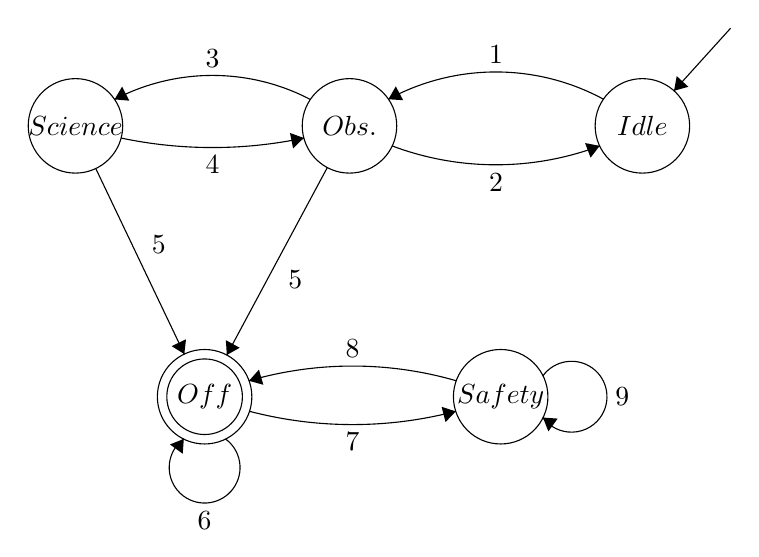
\begin{tikzpicture}[scale=0.2]
\tikzstyle{every node}+=[inner sep=0pt]
\draw [black] (24.2,-19.2) circle (3);
\draw (24.2,-19.2) node {$Obs.$};
\draw [black] (42.8,-19.2) circle (3);
\draw (42.8,-19.2) node {$Idle$};
\draw [black] (6.8,-19.2) circle (3);
\draw (6.8,-19.2) node {$Science$};
\draw [black] (15,-36.4) circle (3);
\draw (15,-36.4) node {$Off$};
\draw [black] (15,-36.4) circle (2.4);
\draw [black] (33.8,-36.4) circle (3);
\draw (33.8,-36.4) node {$Safety$};
\draw [black] (48.4,-13) -- (44.81,-16.97);
\fill [black] (44.81,-16.97) -- (45.72,-16.72) -- (44.98,-16.04);
\draw [black] (26.67,-17.507) arc (118.43354:61.56646:14.344);
\fill [black] (26.67,-17.51) -- (27.61,-17.57) -- (27.14,-16.69);
\draw (33.5,-15.28) node [above] {$1$};
\draw [black] (40.088,-20.475) arc (-69.41442:-110.58558:18.736);
\fill [black] (40.09,-20.47) -- (39.16,-20.29) -- (39.51,-21.22);
\draw (33.5,-22.17) node [below] {$2$};
\draw [black] (9.281,-17.525) arc (117.61533:62.38467:13.416);
\fill [black] (9.28,-17.52) -- (10.22,-17.6) -- (9.76,-16.71);
\draw (15.5,-15.5) node [above] {$3$};
\draw [black] (21.303,-19.973) arc (-78.10445:-101.89555:28.152);
\fill [black] (21.3,-19.97) -- (20.42,-19.65) -- (20.62,-20.63);
\draw (15.5,-21.08) node [below] {$4$};
\draw [black] (8.09,-21.91) -- (13.71,-33.69);
\fill [black] (13.71,-33.69) -- (13.82,-32.75) -- (12.91,-33.19);
\draw (11.61,-26.74) node [right] {$5$};
\draw [black] (16.323,-39.08) arc (54:-234:2.25);
\draw (15,-43.65) node [below] {$6$};
\fill [black] (13.68,-39.08) -- (12.8,-39.43) -- (13.61,-40.02);
\draw [black] (22.79,-21.85) -- (16.41,-33.75);
\fill [black] (16.41,-33.75) -- (17.23,-33.29) -- (16.35,-32.81);
\draw (20.28,-28.97) node [right] {$5$};
\draw [black] (30.948,-37.326) arc (-75.33467:-104.66533:25.865);
\fill [black] (30.95,-37.33) -- (30.05,-37.04) -- (30.3,-38.01);
\draw (24.4,-38.67) node [below] {$7$};
\draw [black] (17.821,-35.385) arc (106.14932:73.85068:23.653);
\fill [black] (17.82,-35.39) -- (18.73,-35.64) -- (18.45,-34.68);
\draw (24.4,-33.95) node [above] {$8$};
\draw [black] (36.48,-35.077) arc (144:-144:2.25);
\draw (41.05,-36.4) node [right] {$9$};
\fill [black] (36.48,-37.72) -- (36.83,-38.6) -- (37.42,-37.79);
\end{tikzpicture}
\end{center}
\begin{center}
Diagram of software states of operation and transition between states.

Transitions between states occur as numbered:

\begin{enumerate}
\item{\textbf{Appogee is reached.} The software shall activate when the power line goes to high at 28V. Observation mode shall be triggered when the OBC turns on.}
\item{\textbf{Error: Return to Idle.} If an error is encountered in entering Observation mode, the software shall fallback to Idle mode and retry. An error may occur if the payload fails to deploy correctly or if the camera fails to turn on.}
\item{\textbf{Payload Assembly and Camera have been deployed.} The software shall enter science mode once the payload assembly and arm have deployed and the camera has performed an observation sweep.}
\item{\textbf{Error: Return to Observation} The software shall return to observation mode if any error occurs in Science mode. An error may occur in Science mode if the arm fails to operate correctly and must return to default position. An error may also occur if the camera stops working.}
\item{\textbf{Timer switches to end appogee period.} Once the time period for observation has ended, the timer line will go to low and trigger to Shutdown state. This state can be reached from either Observation or Science mode.}
\item{\textbf{Accept: Shutdown correctly} If Shutdown occurs correctly, the arm should be closed, the Arm Assembly Body should be retracted, and the OBC should be powered off.}
\item{\textbf{Error: Shutdown not completed successfully.} If an error occurs in the shutdown sequence, the software shall enter Safety mode.}
\item{\textbf{Payload is Shutdown correctly.} If the payload is Shutdown through Safety mode, shutdown can be completed. In Safety mode the payload was either shut down correctly, retracted fully into the can with the arm open, or the arm was expelled safely from the rocket.}
\item{\textbf{Error: Payload is still deployed.} The software shall remain in Safety mode until the payload is either retracted correctly, retracted fully with the arm in the open position, or ejected safely from the rocket. Safety mode shall first try to correctly retract the arm, then retract with the arm open, then repeat attempting ejection until the payload is ejected.}
\end{enumerate}

\subsection{Model of Payload Hardware}
\subsection{Payload Wiring Diagram}
\subsection{References}

\end{document}
\end{center}


\end{document}
